\documentclass{standalone}
\usepackage{tikz}
\usetikzlibrary{patterns, positioning}

\begin{document}
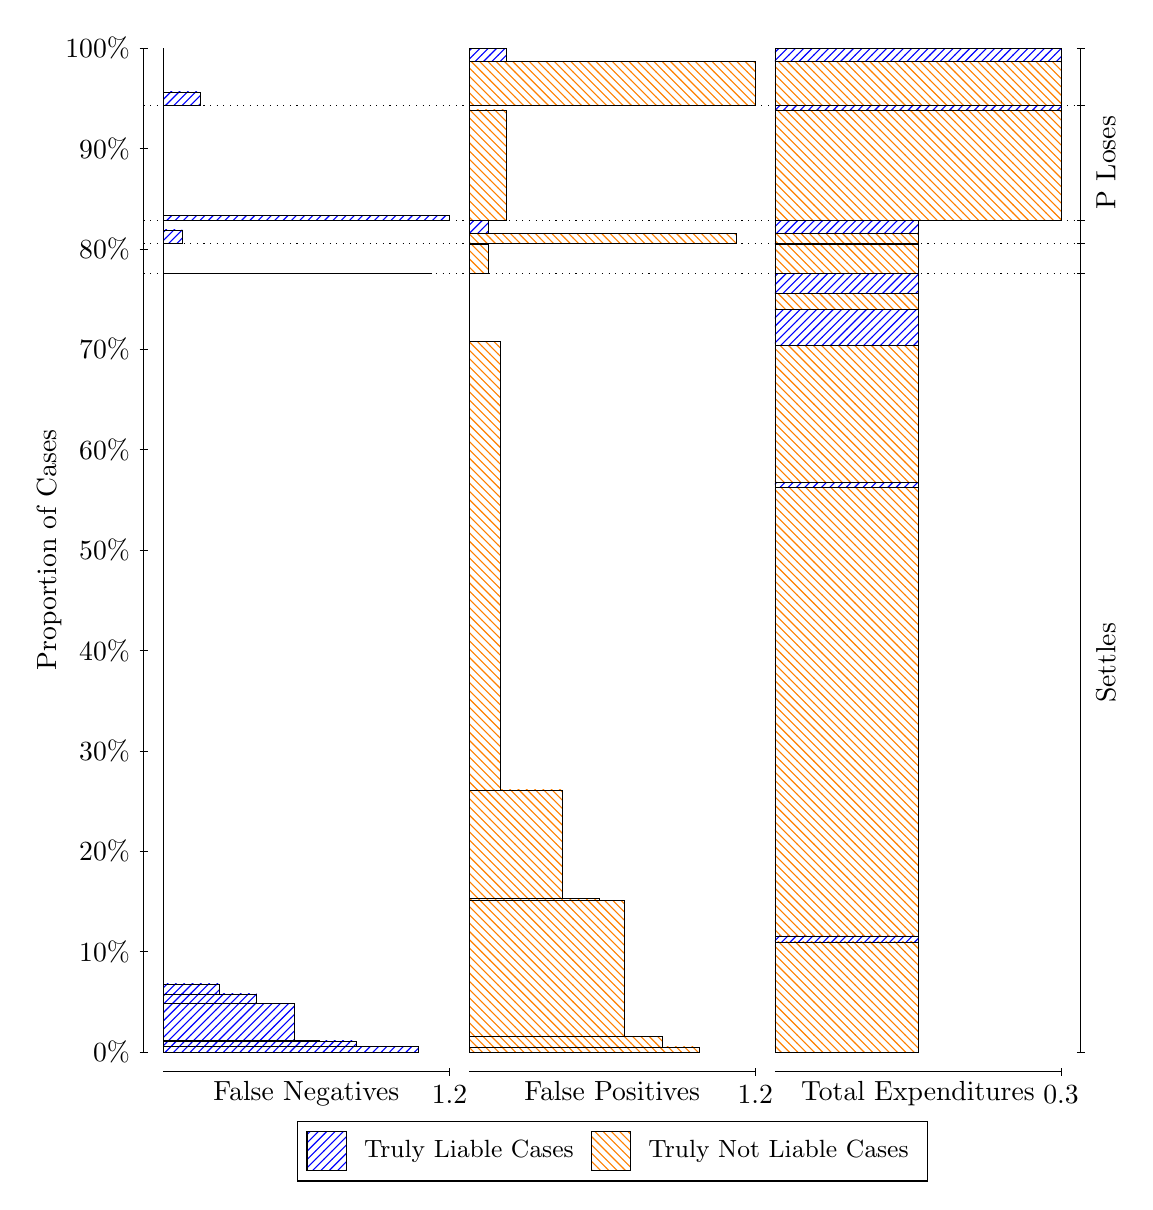
\begin{tikzpicture}
\draw[black, very thin] (1.5,1.75) -- (1.5,14.5);
\node[rotate=90, anchor=center] at (0.3, 8.125) {Proportion of Cases};
\draw[black, very thin] (1.45,1.75) -- (1.55,1.75);
\node[anchor=east] at (1.45, 1.75) {0\%};
\draw[black, very thin] (1.45,3.025) -- (1.55,3.025);
\node[anchor=east] at (1.45, 3.025) {10\%};
\draw[black, very thin] (1.45,4.3) -- (1.55,4.3);
\node[anchor=east] at (1.45, 4.3) {20\%};
\draw[black, very thin] (1.45,5.575) -- (1.55,5.575);
\node[anchor=east] at (1.45, 5.575) {30\%};
\draw[black, very thin] (1.45,6.85) -- (1.55,6.85);
\node[anchor=east] at (1.45, 6.85) {40\%};
\draw[black, very thin] (1.45,8.125) -- (1.55,8.125);
\node[anchor=east] at (1.45, 8.125) {50\%};
\draw[black, very thin] (1.45,9.4) -- (1.55,9.4);
\node[anchor=east] at (1.45, 9.4) {60\%};
\draw[black, very thin] (1.45,10.675) -- (1.55,10.675);
\node[anchor=east] at (1.45, 10.675) {70\%};
\draw[black, very thin] (1.45,11.95) -- (1.55,11.95);
\node[anchor=east] at (1.45, 11.95) {80\%};
\draw[black, very thin] (1.45,13.225) -- (1.55,13.225);
\node[anchor=east] at (1.45, 13.225) {90\%};
\draw[black, very thin] (1.45,14.5) -- (1.55,14.5);
\node[anchor=east] at (1.45, 14.5) {100\%};

\draw[black, very thin] (13.4,1.75) -- (13.4,14.5);
\draw[black, very thin] (13.35,1.75) -- (13.45,1.75);
\node[anchor=west] at (13.35, 1.75) {};
\draw[black, very thin] (13.35,11.634) -- (13.45,11.634);
\node[anchor=west] at (13.35, 11.634) {};
\draw[black, very thin] (13.35,12.019) -- (13.45,12.019);
\node[anchor=west] at (13.35, 12.019) {};
\draw[black, very thin] (13.35,12.315) -- (13.45,12.315);
\node[anchor=west] at (13.35, 12.315) {};
\draw[black, very thin] (13.35,13.775) -- (13.45,13.775);
\node[anchor=west] at (13.35, 13.775) {};
\draw[black, very thin] (13.35,14.5) -- (13.45,14.5);
\node[anchor=west] at (13.35, 14.5) {};

\draw[black, very thin, pattern color=blue, pattern=north east lines] (1.75,1.75) rectangle (4.9884,1.8211);
\draw[black, very thin, pattern color=blue, pattern=north east lines] (1.75,1.8211) rectangle (4.1986,1.8922);
\draw[black, very thin, pattern color=blue, pattern=north east lines] (1.75,1.8922) rectangle (3.7246,1.8981);
\draw[black, very thin, pattern color=blue, pattern=north east lines] (1.75,1.8981) rectangle (3.4087,2.3643);
\draw[black, very thin, pattern color=blue, pattern=north east lines] (1.75,2.3643) rectangle (2.9348,2.4877);
\draw[black, very thin, pattern color=blue, pattern=north east lines] (1.75,2.4877) rectangle (2.4609,2.6142);
\draw[black, very thin, pattern color=orange, pattern=north west lines] (1.75,2.6142) rectangle (1.75,11.634);
\draw[black, very thin, pattern color=blue, pattern=north east lines] (1.75,11.634) rectangle (5.1464,11.642);
\draw[black, very thin, pattern color=orange, pattern=north west lines] (1.75,11.642) rectangle (1.75,12.019);
\draw[black, very thin, pattern color=blue, pattern=north east lines] (1.75,12.019) rectangle (1.987,12.191);
\draw[black, very thin, pattern color=orange, pattern=north west lines] (1.75,12.191) rectangle (1.75,12.315);
\draw[black, very thin, pattern color=blue, pattern=north east lines] (1.75,12.315) rectangle (5.3833,12.376);
\draw[black, very thin, pattern color=orange, pattern=north west lines] (1.75,12.376) rectangle (1.75,13.775);
\draw[black, very thin, pattern color=blue, pattern=north east lines] (1.75,13.775) rectangle (2.2239,13.944);
\draw[black, very thin, pattern color=orange, pattern=north west lines] (1.75,13.944) rectangle (1.75,14.5);
\draw[black, very thin, pattern color=orange, pattern=north west lines] (5.6333,1.75) rectangle (8.5558,1.8159);
\draw[black, very thin, pattern color=orange, pattern=north west lines] (5.6333,1.8159) rectangle (8.0819,1.9491);
\draw[black, very thin, pattern color=orange, pattern=north west lines] (5.6333,1.9491) rectangle (7.608,3.6799);
\draw[black, very thin, pattern color=orange, pattern=north west lines] (5.6333,3.6799) rectangle (7.292,3.705);
\draw[black, very thin, pattern color=orange, pattern=north west lines] (5.6333,3.705) rectangle (6.8181,5.0773);
\draw[black, very thin, pattern color=orange, pattern=north west lines] (5.6333,5.0773) rectangle (6.0283,10.77);
\draw[black, very thin, pattern color=blue, pattern=north east lines] (5.6333,10.77) rectangle (5.6333,11.634);
\draw[black, very thin, pattern color=orange, pattern=north west lines] (5.6333,11.634) rectangle (5.8703,12.011);
\draw[black, very thin, pattern color=blue, pattern=north east lines] (5.6333,12.011) rectangle (5.6333,12.019);
\draw[black, very thin, pattern color=orange, pattern=north west lines] (5.6333,12.019) rectangle (9.0297,12.143);
\draw[black, very thin, pattern color=blue, pattern=north east lines] (5.6333,12.143) rectangle (5.8703,12.315);
\draw[black, very thin, pattern color=orange, pattern=north west lines] (5.6333,12.315) rectangle (6.1072,13.713);
\draw[black, very thin, pattern color=blue, pattern=north east lines] (5.6333,13.713) rectangle (5.6333,13.775);
\draw[black, very thin, pattern color=orange, pattern=north west lines] (5.6333,13.775) rectangle (9.2667,14.331);
\draw[black, very thin, pattern color=blue, pattern=north east lines] (5.6333,14.331) rectangle (6.1072,14.5);
\draw[black, very thin, pattern color=orange, pattern=north west lines] (9.5167,1.75) rectangle (11.333,3.1474);
\draw[black, very thin, pattern color=blue, pattern=north east lines] (9.5167,3.1474) rectangle (11.333,3.2245);
\draw[black, very thin, pattern color=orange, pattern=north west lines] (9.5167,3.2245) rectangle (11.333,8.9173);
\draw[black, very thin, pattern color=blue, pattern=north east lines] (9.5167,8.9173) rectangle (11.333,8.9884);
\draw[black, very thin, pattern color=orange, pattern=north west lines] (9.5167,8.9884) rectangle (11.333,10.719);
\draw[black, very thin, pattern color=blue, pattern=north east lines] (9.5167,10.719) rectangle (11.333,11.185);
\draw[black, very thin, pattern color=orange, pattern=north west lines] (9.5167,11.185) rectangle (11.333,11.384);
\draw[black, very thin, pattern color=blue, pattern=north east lines] (9.5167,11.384) rectangle (11.333,11.634);
\draw[black, very thin, pattern color=orange, pattern=north west lines] (9.5167,11.634) rectangle (11.333,12.011);
\draw[black, very thin, pattern color=blue, pattern=north east lines] (9.5167,12.011) rectangle (11.333,12.019);
\draw[black, very thin, pattern color=orange, pattern=north west lines] (9.5167,12.019) rectangle (11.333,12.143);
\draw[black, very thin, pattern color=blue, pattern=north east lines] (9.5167,12.143) rectangle (11.333,12.315);
\draw[black, very thin, pattern color=orange, pattern=north west lines] (9.5167,12.315) rectangle (13.15,13.713);
\draw[black, very thin, pattern color=blue, pattern=north east lines] (9.5167,13.713) rectangle (13.15,13.775);
\draw[black, very thin, pattern color=orange, pattern=north west lines] (9.5167,13.775) rectangle (13.15,14.331);
\draw[black, very thin, pattern color=blue, pattern=north east lines] (9.5167,14.331) rectangle (13.15,14.5);
\draw[black, dotted] (1.5,11.634) -- (13.4,11.634);
\draw[black, dotted] (1.5,12.019) -- (13.4,12.019);
\draw[black, dotted] (1.5,12.315) -- (13.4,12.315);
\draw[black, dotted] (1.5,13.775) -- (13.4,13.775);
\draw[black, very thin] (1.75,1.5) -- (5.3833,1.5);
\node[anchor=north] at (3.5667, 1.5) {False Negatives};
\draw[black, very thin] (5.3833,1.45) -- (5.3833,1.55);
\node[anchor=north] at (5.3833, 1.45) {1.2};

\draw[black, very thin] (5.6333,1.5) -- (9.2667,1.5);
\node[anchor=north] at (7.45, 1.5) {False Positives};
\draw[black, very thin] (9.2667,1.45) -- (9.2667,1.55);
\node[anchor=north] at (9.2667, 1.45) {1.2};

\draw[black, very thin] (9.5167,1.5) -- (13.15,1.5);
\node[anchor=north] at (11.333, 1.5) {Total Expenditures};
\draw[black, very thin] (13.15,1.45) -- (13.15,1.55);
\node[anchor=north] at (13.15, 1.45) {0.3};

\node[black, centered, rotate=90] at (13.72, 6.6921) {Settles};


\node[black, centered, rotate=90] at (13.72, 13.045) {P Loses};


\draw (7.449999999999999,1.5) node[draw=none] (baseCoordinate) {};
\begin{scope}[align=center]
        \matrix[scale=0.5, draw=black, below=0.5cm of baseCoordinate, nodes={draw}, column sep=0.1cm]{
            \node[rectangle, draw, minimum width=0.5cm, minimum height=0.5cm, pattern=north east lines, pattern color=blue] {}; &
            \node[draw=none, font=\small] (B) {Truly Liable Cases}; &
            \node[rectangle, draw, minimum width=0.5cm, minimum height=0.5cm, pattern=north west lines, pattern color=orange] {}; &
            \node[draw=none, font=\small] (B) {Truly Not Liable Cases}; \\
            };
\end{scope}

\end{tikzpicture}
\end{document}